\section{Modeling}\label{sec:modeling}
In order to model the Jao Gap we evolve two extremely finely sampled mass grids
of models. One of these grids uses the OPAL high-temperature opacity tables
while the other uses the OPLIB tables (Figure \ref{fig:PunchIn}). Each grid
evolves a model every 0.00025 $M_{\odot}$ from 0.2 to 0.4 $M_{\odot}$ and every
0.005 $M_{\odot}$ from 0.4 to 0.8 $M_{\odot}$. All models in both grids use a
GS98 solar composition, the (1, 101, 0) \texttt{FreeEOS} (version
{\color{red}2.7}) configuration, and 1000 year old pre-main sequence polytropic
models, with polytropic index 1.5, as their initial conditions. We
include gravitational settling in our models where elements are grouped
together. Finally, we set a maximum allowed timestep of 50 million years to
assure that we fully resolve the build of of core $^{3}$He in gap stars.

Despite the alternative view of convection provided by
\citet{MacDonald2018} discussed in Section \ref{sec:JaoGap}, given that the
mixing timescales in these low mass stars are so short \citep[between $10^{7}$s
and $10^{8}$s per][Figure 2 \& Equation 39, which present the
averaged velocity over the convection zone]{Jermyn2022} instantaneous mixing is a valid
approximation. Moreover, one principal motivation for a diffusive model of
convective mixing has been to account for a deuterium concentration gradient
which \citet{Chabrier1997} identify will develop when the deuterium lifetime
against proton capture is significantly shorter than the mixing timescale.
However, the treatment of energy generation used by DSEP \citep{Bahcall2001}
avoides this issue by computing both the equilibrium deuterium abundance and
luminosity of each shell individually, implicitly accounting for the overall
luminosity discrepancy identified by \citeauthor{Chabrier1997}.

Because in this work we are just interested in the location shift of the Gap as
the opacity source varies, we do not model variations in composition.
\citet{Mansfield2021,Jao2020,Feiden2021} all look at the effect composition has
on Jao Gap location. They find that as population metallicity increases so too
does the mass range and consequently the magnitude of the Gap. From an extremely
low metallicity population (Z=0.001) to a population with a more solar like
metallicity this shift in mass range can be up to 0.05 M$_{\odot}$
\citep{Mansfield2021}.

\begin{figure}
	\centering
	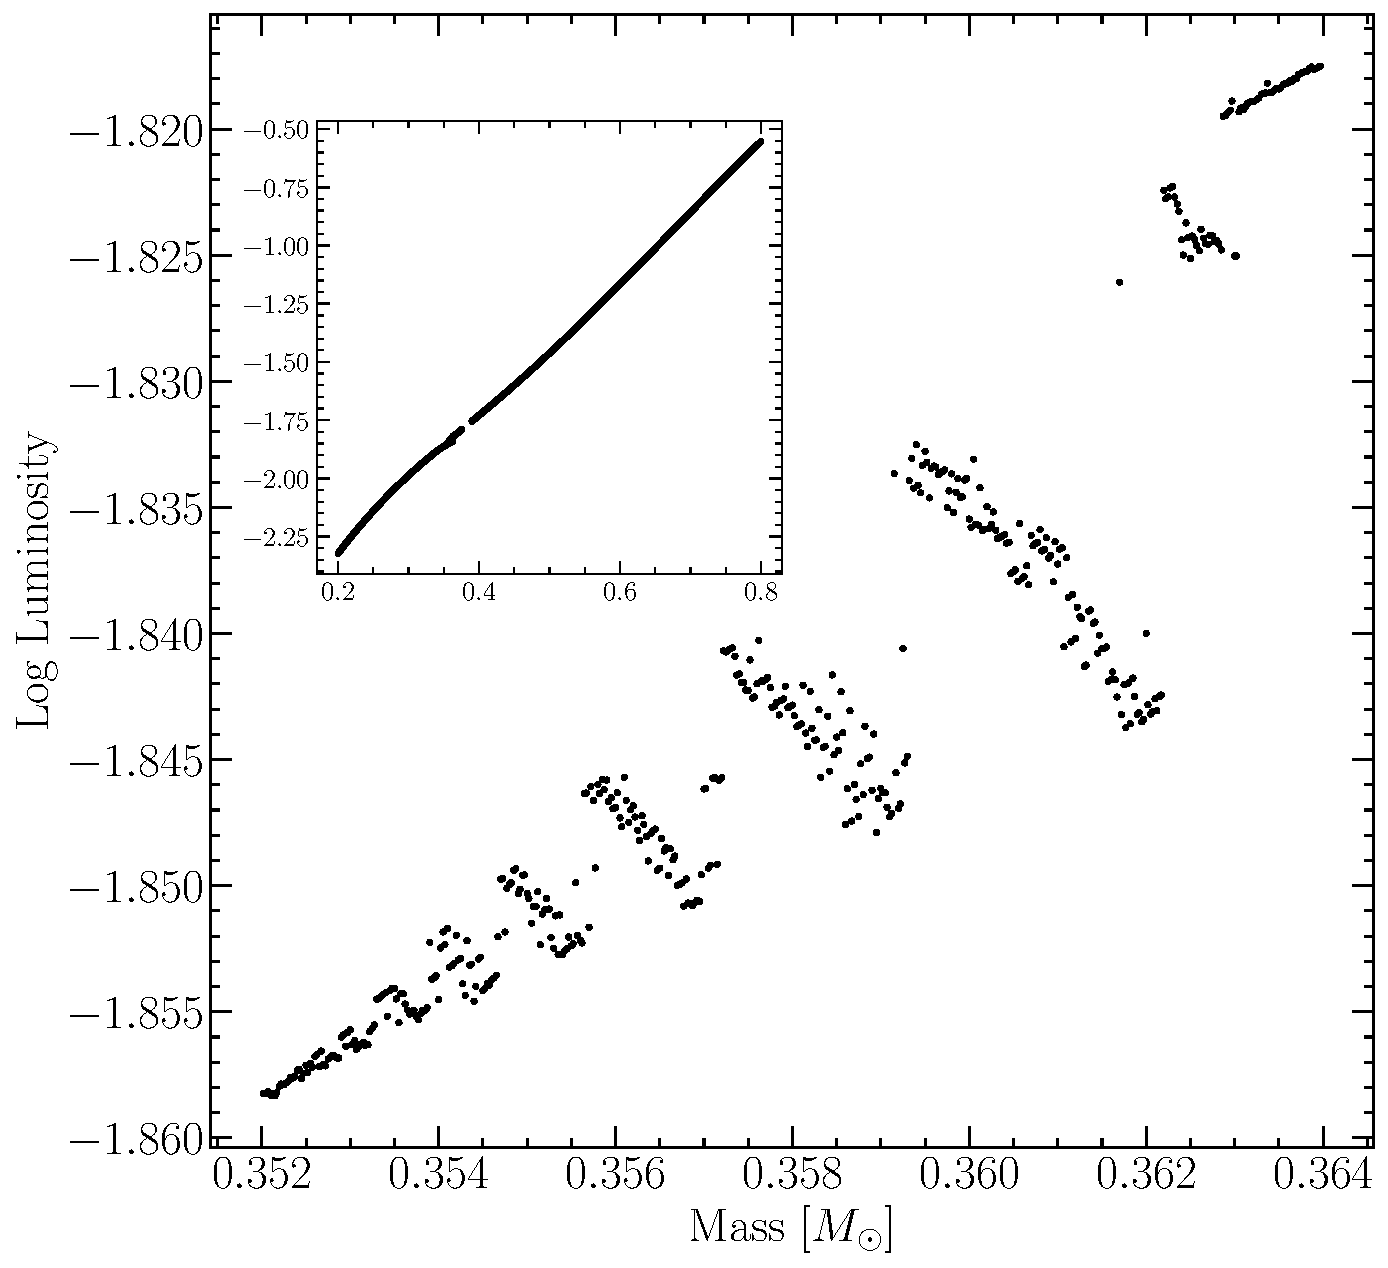
\includegraphics[width=0.85\textwidth]{figures/jaoOpacity/OPALPunchIn.pdf}
	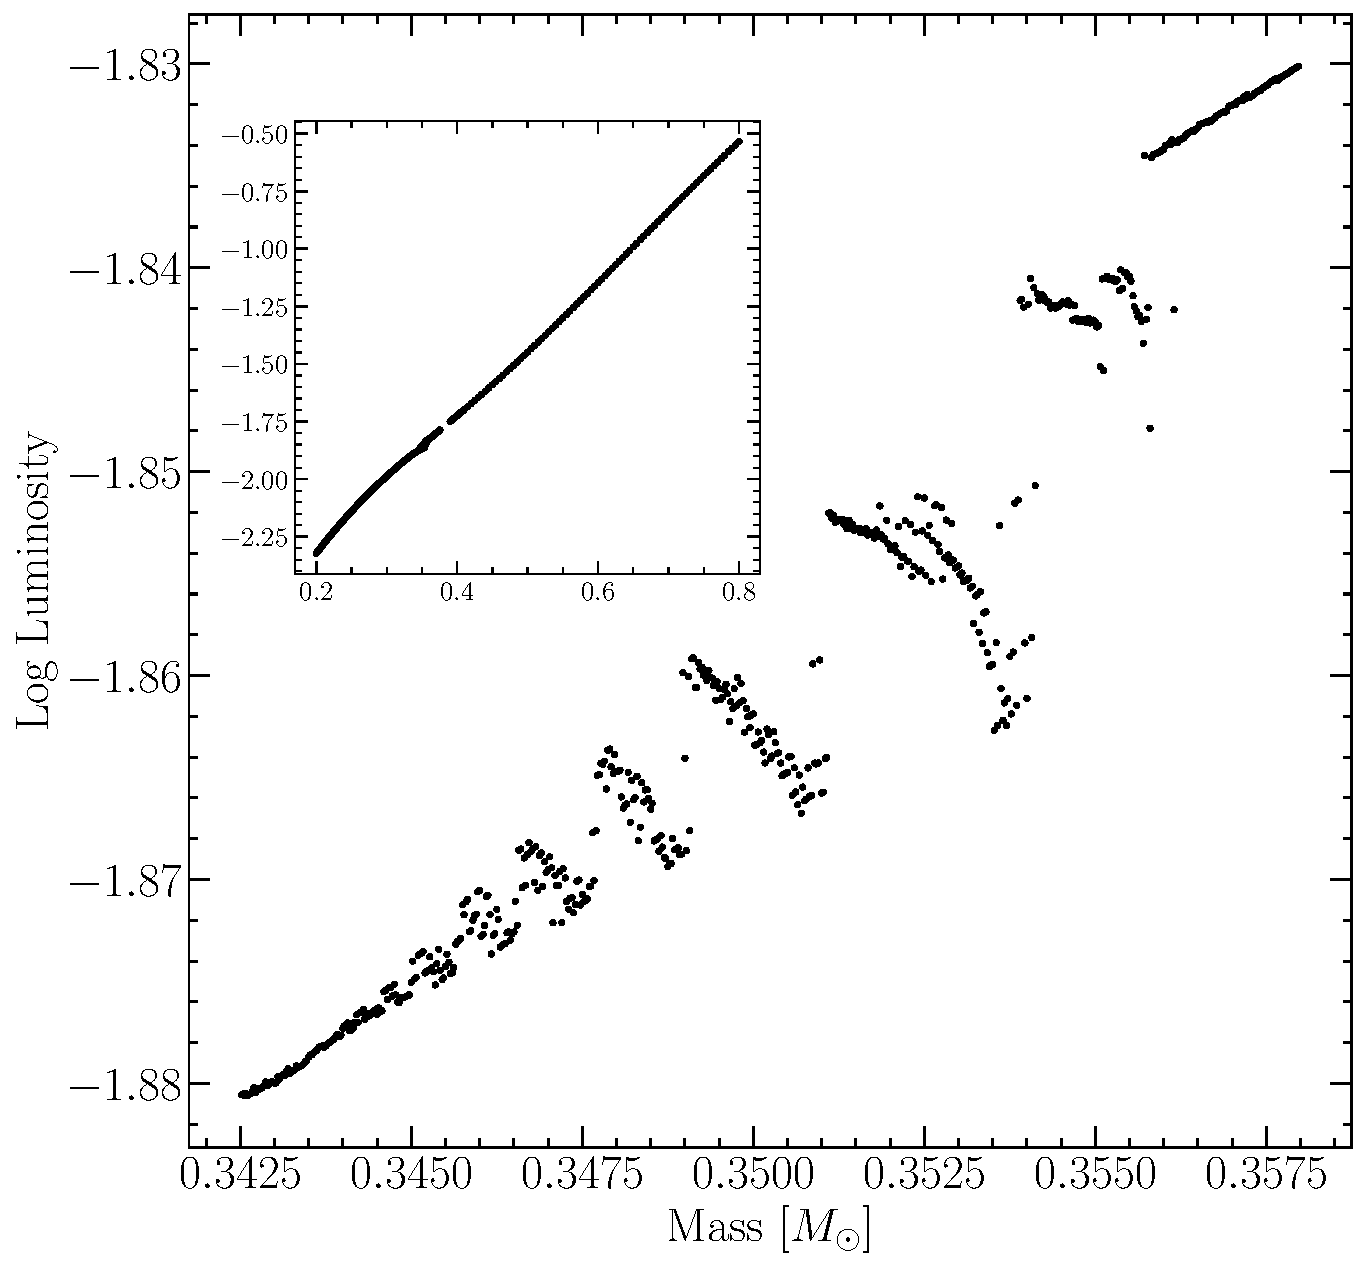
\includegraphics[width=0.85\textwidth]{figures/jaoOpacity/OPLIBPunchIn.pdf}
	\caption{Mass-luminosity relation at 7 Gyrs for models evolved using OPAL opacity
	tables (top) and those evolved using OPLIB opacity tables (bottom). Note
	the lower mass range of the OPLIB Gap.}
	\label{fig:PunchIn}
		
\end{figure}

\subsection{Population Synthesis}
In order to compare the Gap to observations we use in house population
synthesis code. We empirically calibrate the relation between G, BP, and RP
magnitudes and their uncertainties along with the parallax/G magnitude
uncertainty relation using the Gaia Catalouge of Nearby Stas
\citep[GCNS,][]{GaiaCollaboration2021} and Equations \ref{eqn:plxCalib} \&
\ref{eqn:MagCalib}. $M_{g}$ is the Gaia G magnitude while $M_{i}$ is the
magnitude in the i$^\text{th}$ band, G, BP, or RP. The coefficients $a$, $b$,
and $c$ determined using a non-linear least squares fitting routine. Equation
\ref{eqn:plxCalib} then models the relation between G magnitude and parallax
uncertainty while Equation \ref{eqn:MagCalib} models the relation between each
magnitude and its uncertainty.

\begin{align}\label{eqn:plxCalib}
	\sigma_{plx}(M_{g}) = ae^{bM_{g}}+c
\end{align}
\begin{align}\label{eqn:MagCalib}
	\sigma_{i}(M_{i}) = ae^{M_{i}-b}+c
\end{align}

\noindent The full series of steps in our population synthesis code
are:

\begin{figure}
	\centering
	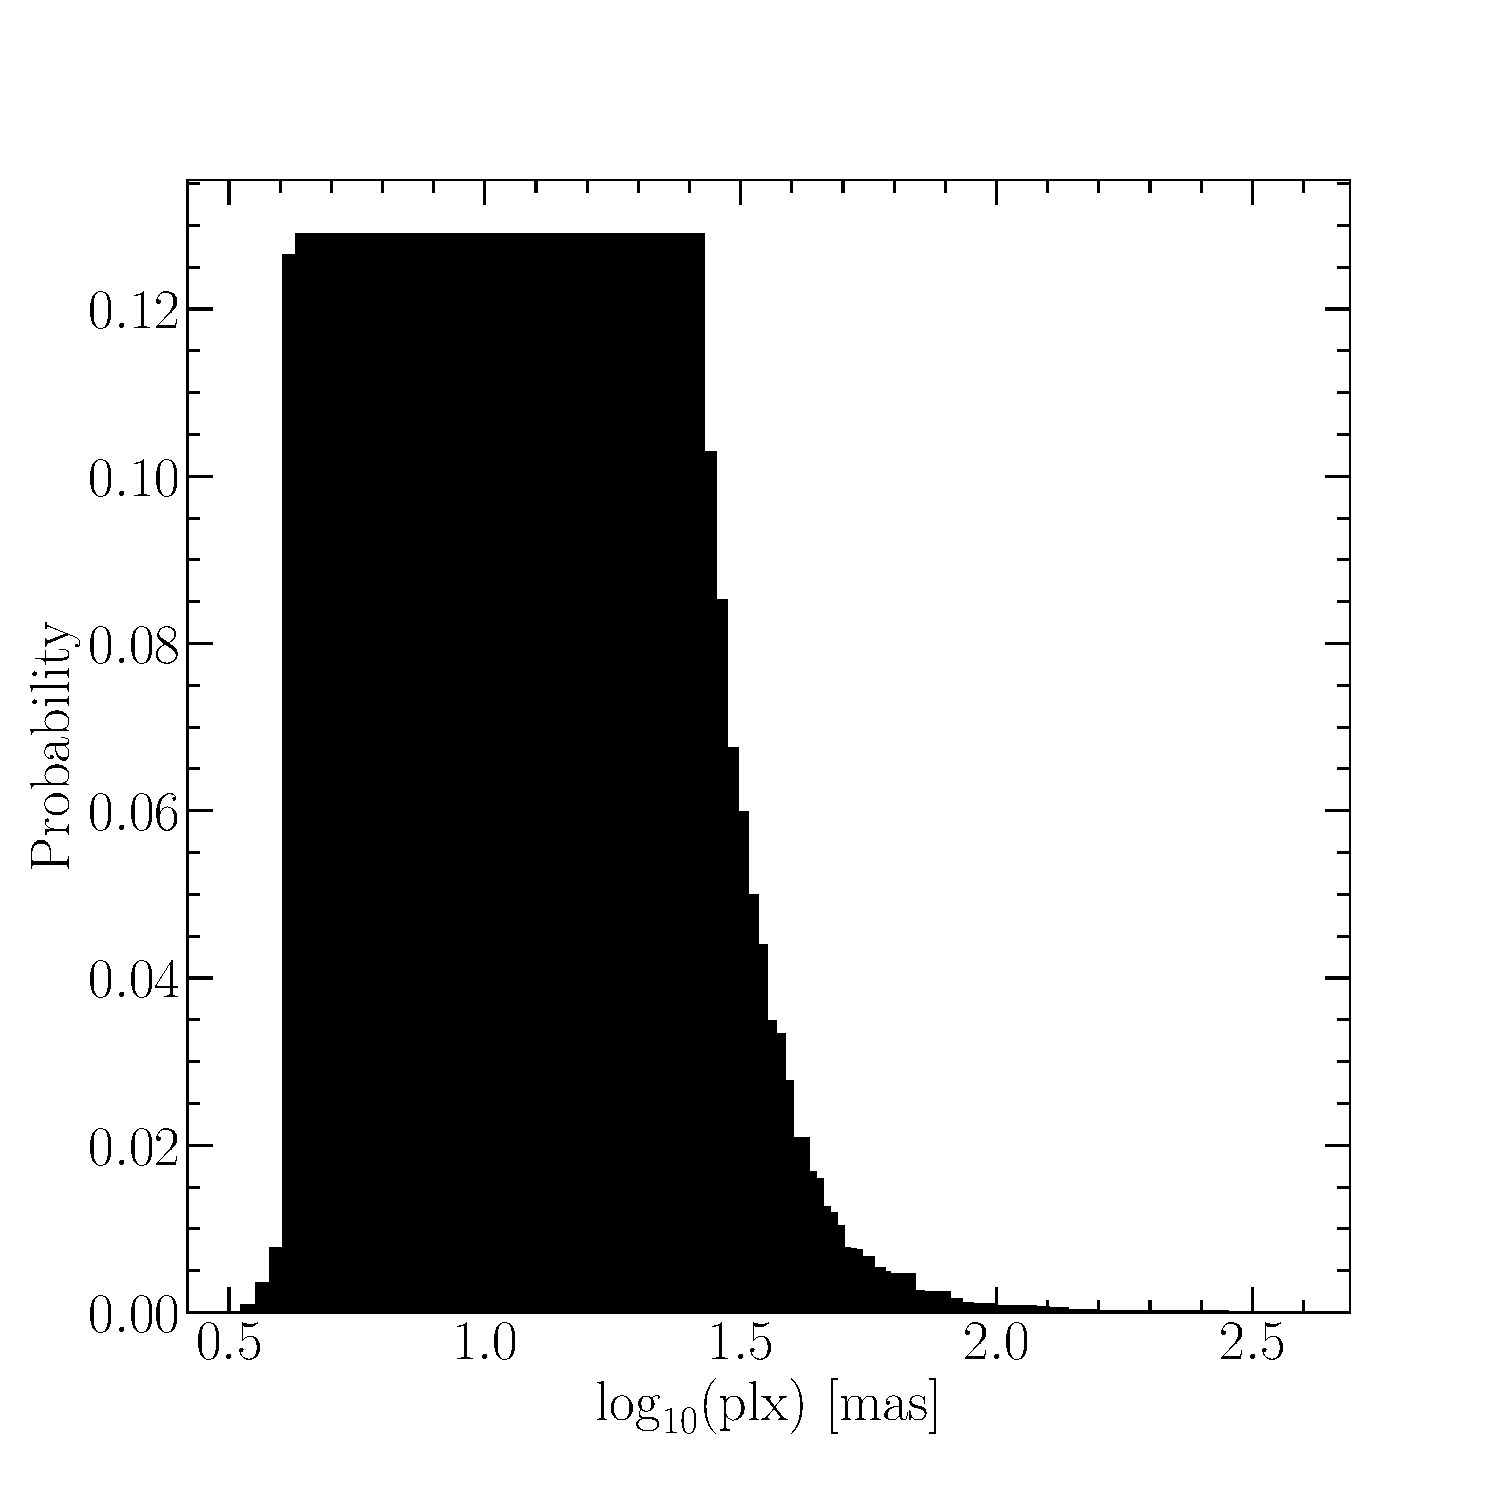
\includegraphics[width=0.85\textwidth]{figures/jaoOpacity/pdist.pdf}
	\caption{Probability distribution sampled when assigning true parallaxes to
	synthetic stars. This distribution is built from the GCNS and includes all
	stars with BP-RP colors between 2.3 and 2.9, the same color range
	of the Jao Gap.}
	\label{fig:pdist}
\end{figure}

\begin{enumerate}
	\item Sample from a \citet{Sollima2019} ($0.25 M_{\odot} < M < 1 M_{\odot}$,
		$\alpha=-1.34\pm0.07$) IMF to determine synthetic star mass.
	\item Find the closest model above and below the synthetic star, lineally
		interpolate these models' $T_{eff}$, $\log(g)$, and $\log(L)$ to those
		at the synthetic star mass.
	\item Convert synthetic star $g$, $T_{eff}$, and $Log(L)$ to Gaia G, BP,
		and RP magnitudes using the Gaia (E)DR3 bolometric corrections
		\citep{Creevey2022} along with code obtained thorough personal
		communication with Aaron Dotter \citep{Choi2016}.
	\item Sample from the GCNS parallax distribution (Figure \ref{fig:pdist}),
		limited to stars within the BP-RP color range of 2.3 -- 2.9, to assign
		synthetic star a ``true'' parallax.
	\item Use the true parallax to find an apparent magnitude for each filter.
	\item Evaluate the empirical calibration given in Equation
		\ref{eqn:plxCalib} to find an associated parallax uncertainty. Then
		sample from a normal distribution with a standard deviation equal to
		that uncertainty to adjust the true parallax resulting in an
		``observed'' parallax.
	\item Use the ``observed'' parallax and the apparent magnitude to find an
		``observed'' magnitude.
	\item Fit the empirical calibration given in Equation \ref{eqn:MagCalib} to
		the GCNS and evaluate it to give a magnitude uncertainty scale in each
		band.
	\item Adjust each magnitude by an amount sampled from a normal
		distribution with a standard deviation of the magnitude uncertainty
		scale found in the previous step.
\end{enumerate}

This method then incorporates both photometric and astrometric uncertainties
into our population synthesis. An example 7 Gyr old synthetic populations
using OPAL and OPLIB opacities are presented in Figure
\ref{fig:PopSynthCompareBasic}.

\begin{figure*}
	\centering
	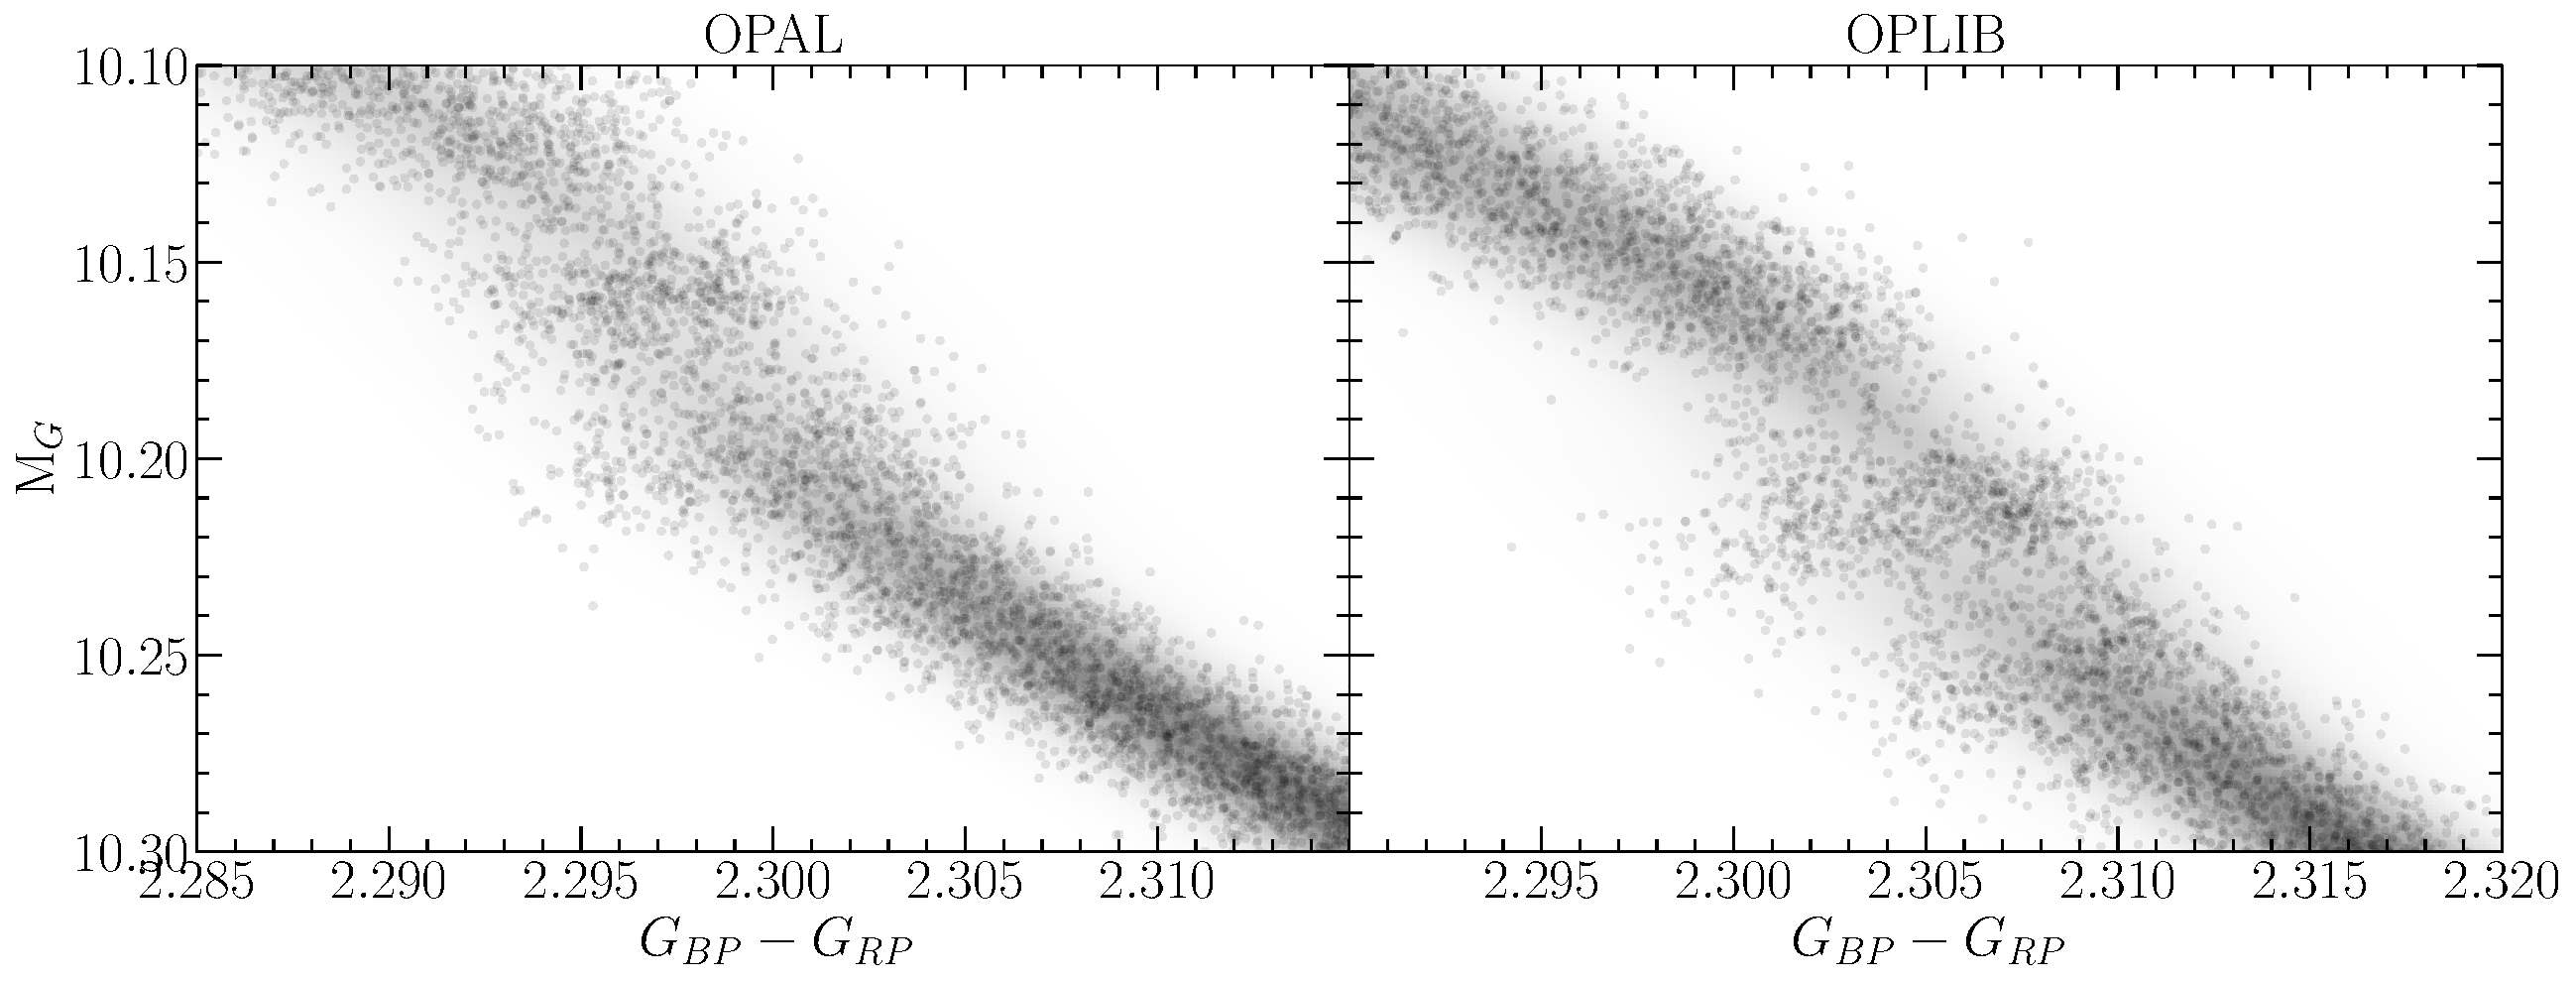
\includegraphics[width=0.85\textwidth]{figures/jaoOpacity/OPALOPLIB_popsynth_compare.pdf}
	\caption{Population synthesis results for models evolved with OPAL (left)
	and models evolved with OPLIB (right). A Gaussian kernel-density estimate
	has been overlaid to better highlight the density variations.}
	\label{fig:PopSynthCompareBasic}
\end{figure*}

\subsection{Mixing Length Dependence}
In order to test the sensitivity of Gap properties to mixing length we
evolve three separate sets OPLIB of models. The first uses a GS98
solar calibrated mixing length, the second uses a mixing length of
1.5, and the third uses a mixing length of 1.0.

We find a clear inverse correlation between mixing length parameter used and
the magnitude of the Jao Gap Figures \ref{fig:MixingLengthCMD} \&
\ref{fig:MixingLengthScaling} ($\mu_{G} \propto -1.5\alpha_{ML}$, where
$\mu_{G}$ is the mean magnitude of the Gap). This is somewhat surprising given
the long established view that the mixing length parameter is of little
relevance in fully convective stars \citep{Baraffe1997}. We find an approximate
0.3 magnitude shift in both the color and magnitude comparing a solar
calibrated mixing length to a mixing length of 1.5, despite only a 16K
difference in effective temperature at 7Gyr between two 0.3 solar mass models.
The slight temperature differences between these models are
attributable to the steeper adiabatic temperature gradients just below the
atmosphere in the solar calibrated mixing length model compared to the
$\alpha_{ML} = 1.5$ model ($\nabla_{ad,solar} - \nabla_{ad,1.5} \approx 0.05$).
Despite this relatively small temperature variance, the large magnitude
difference is expected due to the extreme sensitivity of the bolometric
corrections on effective temperature at these low temperatures. The
mixing length then provides a free parameter which may be used to shift the gap
location in order to better match observations without having a major impact on
the effective temperature of models. Moreover, recent work indicates that using
a solar calibrated mixing length is not appropriate for all stars
\citep[e.g.][]{Trampedach2014, Joyce2018}.

\begin{figure}
	\centering
	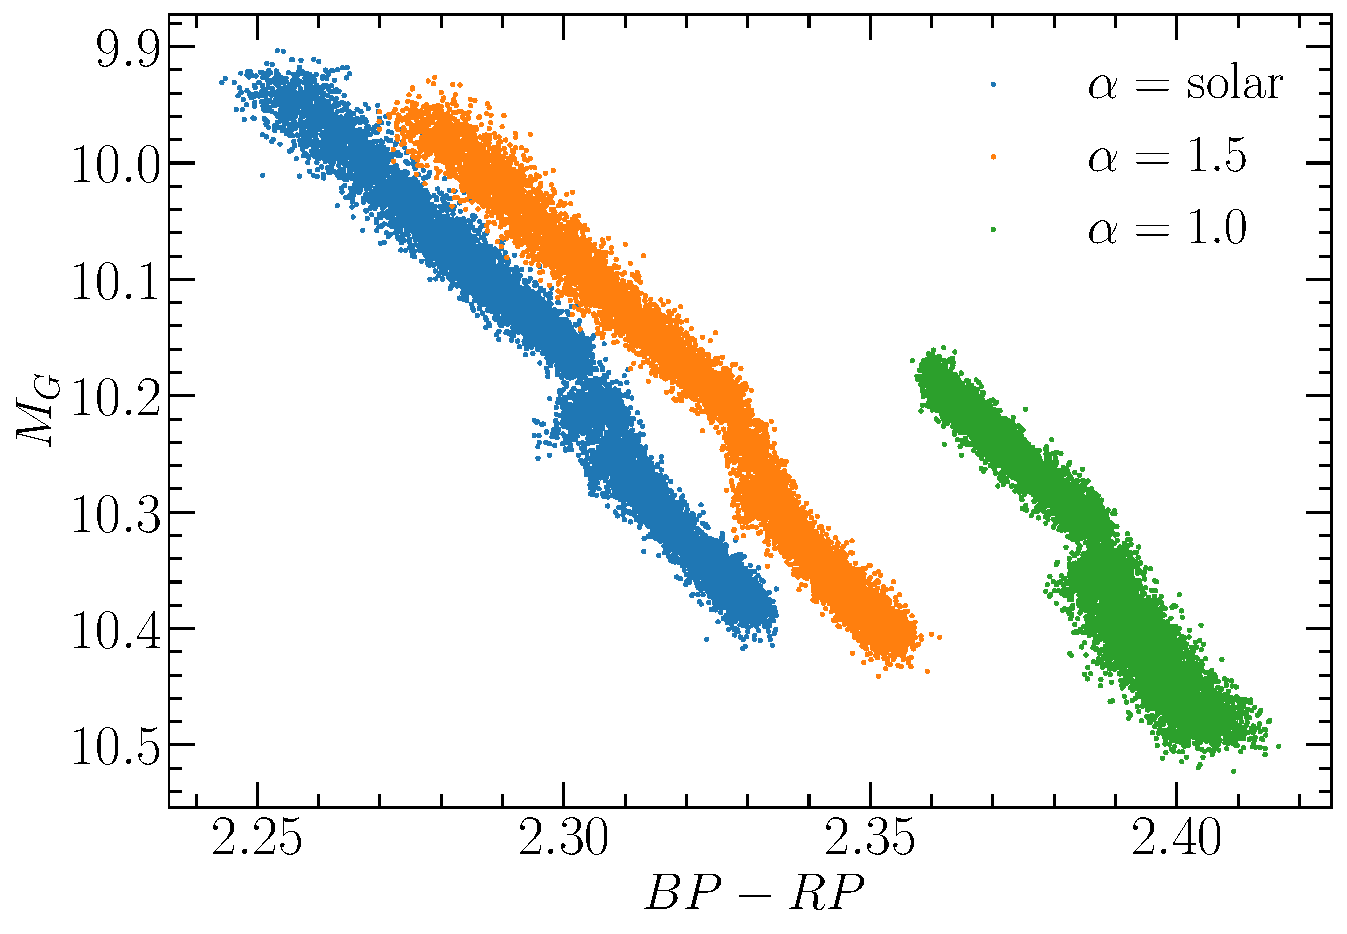
\includegraphics[width=0.85\textwidth]{figures/jaoOpacity/./alphaMLComparisionCMD.pdf}
	\caption{CMD showing OPLIB populations (from left to right) A, B, and C.}
	\label{fig:MixingLengthCMD}
\end{figure}

\begin{figure}
	\centering
	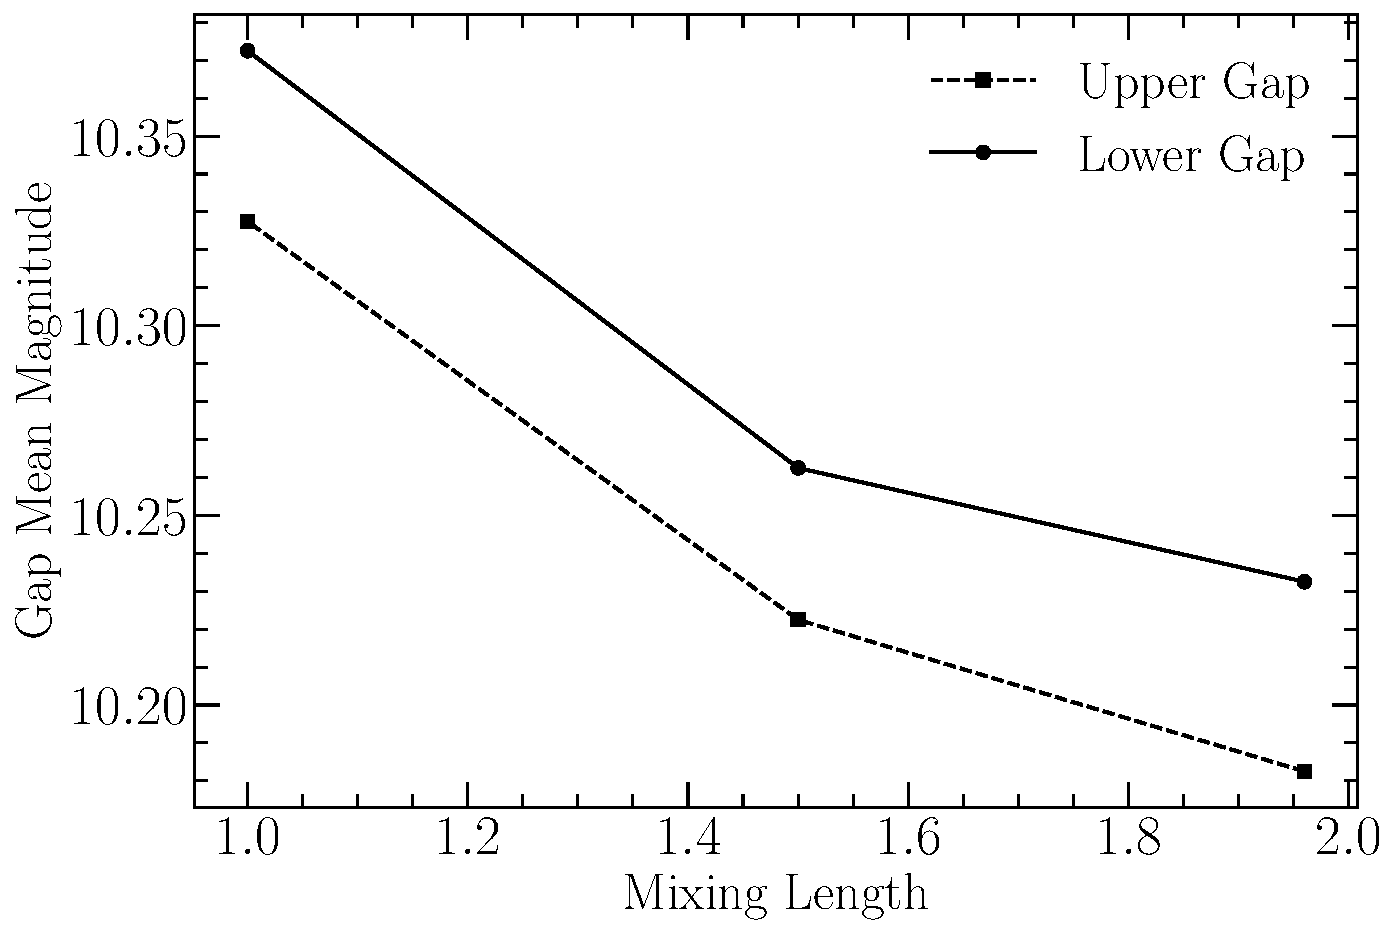
\includegraphics[width=0.85\textwidth]{figures/jaoOpacity/./MixingLengthScaling.pdf}
	\caption{Location of the two identified paucities of stars in OPLIB synthetic
	populations as a function of the mixing length used.}
	\label{fig:MixingLengthScaling}
\end{figure}

Given the variability of gap location with mixing length, it is possible that a
better fit to the gap location may be achieved through adjustment of the
convective mixing length parameter. However, calibrations of the mixing length
for stars other than the sun have focused on stars with effective temperature
at or above that of the sun and there are no current calibrations of the mixing
length parameter for M dwarfs. Moreover, there are additional uncertainties
when comparing the predicted gap location to the measured gap location, such as
those in the conversion from effective temperature, surface gravity, and
luminosity to color, which must be considered if the mixing length is to be
used as a gap location free parameter. Given the dangers of freely adjustable
parameters and the lack of an a priori expectation for what the convective
mixing parameter should be for the population of M Dwarfs in the Gaia DR2 and
EDR3 CMD any attempt to use the Jao Gap magnitude to calibrate a mixing length
value must be done with caution, and take into account the other uncertainties
in the stellar models which could affect the Jao Gap magnitude.

